\subsection{The Dynamic Dijkstra Algorithm}

The first algorithm we discuss is a simple modification of the Dijkstra Algorithm to determine the earliest arrival times $(l_{s,w}(\theta))_{w\in V'}$ at nodes of some subset $V'\subseteq V$ when departing from a source node $s$ at time $\theta$.
Here, only those nodes are relevant for us that are reachable from $s$ and that can reach $t$.
Moreover, we only need to determine the arrival times of nodes $w$ that can be reached before $t$, i.e. that fulfill $l_{s,w}(\theta) \leq l_{s,t}(\theta)$.
Hence, the set $V'$ consists of all nodes $w$ that lie on a path from $v$ to $t$ and fulfill $l_{s,w}(\theta) \leq l_{s,t}(\theta)$.

\begin{algorithm}[ht]
\begin{minted}[mathescape, linenos]{python}
def dynamic_dijkstra(
    theta: float, source: Node, sink: Node, relevant_nodes: Set[Node],
    costs: List[Callable[[float], float]]
) -> Dict[Node, float]:
  arrival_times: Dict[Node, float] = {}
  queue: PriorityQueue[Node] = PriorityQueue([(source, theta)])
  while len(queue) > 0:
    arrival_time, v = queue.min_key(), queue.pop()
    arrival_times[v] = arrival_time
    if v == sink:
      break
    for e in v.outgoing_edges:
      w = e.node_to
      if w in arrival_times.keys() or w not in relevant_nodes:
        continue
      relaxation = arrival_time + costs[e.id](arrival_time)
      if not queue.contains(w):
        queue.push(w, relaxation)
      elif relaxation < queue.key_of(w):
        queue.decrease_key(w, relaxation)
  return arrival_times
\end{minted}
\caption{The Dynamic Dijkstra Algorithm}
\label{alg:dynamic-dijkstra}
\end{algorithm}

Adjusting the classical Dijkstra Algorithm for static edge costs to our setting yields the Dynamic Dijkstra Algorithm as depicted in Algorithm~\ref{alg:dynamic-dijkstra}.

A priority queue, consisting of items together with a priority key associated with each item, operates at the heart of the algorithm.
This queue has to support the operations \code{push(item, key)}, \code{min_key()}, \code{pop()}, \code{decrease_key(item, new_key)} as well as \code{contains(item)}.
The operation \code{push(item, key)} adds the item \code{item} with priority \code{key} to the queue, \code{min_key()} returns the minimum key of an item in the queue, \code{pop()} returns the item with minimum key and removes it from the queue, \code{contains(item)} returns whether \code{item} is contained in the queue and the operation \code{decrease_key(item, new_key)} replaces the priority key associated to the item \code{item} with \code{new_key}.


The idea of Algorithm~\ref{alg:dynamic-dijkstra} is to iteratively retrieve an unvisited node $v$ with the current earliest arrival time $t$ of all unvisited nodes.
Then, for each outgoing edge $e=vw$ we realize its cost at time $t$ and update the arrival time of the target node $w$.
The priority queue holds all discovered but unvisited nodes where the priority key of a node $w$ is its currently suspected earliest arrival time, an upper bound on $l_{s,w}(\theta)$.
Nodes that are not added to the queue have either been already visited and thus have an entry in \code{arrival_times} or are not discovered and hence have an imaginary arrival time of $\infty$.

In the following proposition we show the correctness of the algorithm:

\begin{proposition}
    Given cost functions $c:\R \rightarrow \R_{\geq0}^E$ following the FIFO rule, the Dynamic Dijkstra Algorithm initiated on the source $s\in V$ and a reachable sink $t\in V$ computes the vector $(l_{s,w}(\theta))_{w\in V'}$ with \[
        V' = \{ w\in V \mid \text{$w$ lies on an $s$-$t$-path and $l_{s,w}(\theta) \leq l_{s,t}(\theta)$} \}.
    \]
\end{proposition}
\begin{proof}
    As an invariant for the algorithm we proof, that once a value of a node $w$ is written to \code{arrival_times[w]}, this value coincides with $l_{s,w}(\theta)$.
    In the beginning this is clearly true as \code{arrival_times} is initially empty.
    In the first iteration of the loop, the variable $\code{v}$ holds the source $s$ and its key $\theta= l_{s,s}(\theta)$ is written to \code{arrival_times[v]}.
    Assume the loop invariant holds before entering the body of the loop again at a later time and let $v$ be the popped node.
    As nodes are added at most once to the queue, we have $v \neq s$.
    Let $u$ be the node in whose iteration $v$ was added to the queue or the key of $v$ in the queue was decreased the most recently.
    The invariant implies $\code{arrival_times[}u\code{]} = l_{v,u}(\theta)$ and thus $\code{arrival_time} = l_{s,u}(\theta) + c_{uv}(l_{s,u}(\theta)) = T_{uv}(l_{s,u}(\theta)) \geq l_{s,v}(\theta)$.

    Assume $\code{arrival_time} > l_{s,v}(\theta)$ and let $P$ be a shortest $s$-$v$-path at time $\theta$.
    If all nodes of $P$ were available in \code{arrival_times}, then the last node before $v$ in $P$ would have set the key of $v$ in its iteration to $l_{s,v}(\theta)$.
    Let $u$ be the first node in $P$ that is not available in \code{arrival_times}.
    Because $u$ cannot be the source $s$, the  predecessor $u'$ of $u$ in $P$ must have set the key of $u$ to at most $T_{u'u}(l_{s,u'}(\theta)) \leq T_P(\theta)$.
    As $\code{arrival_time}>l_{s,v}(\theta) = l_P(\theta)$ the key of $u$ in the queue was smaller than the key of $v$, so the priority queue would have popped $u$ before $v$.
\end{proof}

A simple binary min-heap together with a lookup table was implemented to support the operations of the queue efficiently.
With this data structure, the worst case running time is logarithmic in the number of queue items for the operations \code{push(item, key)}, \code{pop()} and \code{decrease_key(item, new_key)} and constant for the operations \code{min_key()} and \code{contains(item)}.
Thus, the Dynamic Dijkstra Algorithm terminates with a running time of $\bigO( (\abs{V} + \abs{E}) \cdot \log \abs{V})$.


\subsection{Computing Active Outgoing Edges}\label{sec:compute-active-edges}

Given a FIFO cost function $c: \R\rightarrow\R_{\geq0}^E$ with nodes $s,t\in V$, a time $\theta\in\R$, we want to compute the active outgoing edges $E(\theta) \cap \outEdges{s}$ of $s$, i.e. the edges $e=sw$ with 
\[
    l_{s,t}(\theta) = l_{w,t}(T_e(\theta)).
\]
Unfortunately, from the arrival times $(l_{s,w}(\theta))_{w\in V'}$ obtained by a simple run of the Dynamic Dijkstra Algorithm, we cannot determine all active edges:
Usually, the idea is to backtrack all shortest paths by searching edges $e=vw$ backwards starting from $t$ for which equality holds in $l_{s,w}(\theta) \leq T_e(l_{s,v}(\theta))$.
This approach is described in Algorithm~\ref{alg:backward-search} which aims to return the set $E(\theta)\cap \outEdges{s}$.
The vector $(l_{s,w}(\theta))_{w\in V'}$ as returned by the Dynamic Dijkstra Algorithm is passed to the function via the parameter \code{arrivals}.
During the procedure, we only enqueue a node $u$ to the queue \code{queue}, if there exists a path from $u$ to $t$ in which each edge $e=vw$ fulfills $l_{s,w}(\theta)= T_e(l_{s,v}(\theta))$.
Once we discover an edge from $s$ to such an enqueued node that also fulfills the equality, we add it to the set of active outgoing edges of $s$ which is returned by the algorithm.

\begin{algorithm}
    \begin{minted}[mathescape, linenos]{python}
def backtrack_shortest_paths(
  costs: List[Callable[[float], float]], arrivals: Dict[Node, float],
  source: Node, sink: Node
) -> Set[Edge]:
  active_edges = set()
  queue: List[Node] = [sink]
  discovered: Set[Node] = {sink}
  while len(queue) > 0:
    w = queue.pop()
    for e in w.incoming_edges:
      v = e.node_from
      if v not in arrivals.keys():
        continue
      if arrivals[v] + costs[e.id](arrivals[v]) <= arrivals[w]:
        if v == source:
          active_edges.add(e)
        if v not in discovered:
          queue.append(v)
          discovered.add(v)
  return active_edges
    \end{minted}
    \caption{Retrieve Active Edges by Backtracking Shortest Paths}
    \label{alg:backward-search}
\end{algorithm}

The following proposition proves that paths found using the described approach are in fact shortest paths.
Moreover, we show that for strong FIFO costs we find all shortest paths.
That means, for strong FIFO costs, Algorithm~\ref{alg:backward-search} returns the whole set $E(\theta)\cap\outEdges{s}$.

\begin{proposition}
    Let $P=e_1\,\cdots\,e_k$ be a path with $e_i = v_{i-1}v_{i}$ and $v_0 = s, v_k= t$ and let $c:\R\rightarrow\R^E_{\geq0}$ be a cost function following the FIFO rule. Then
    \[ 
        \left(\forall i:\, {T_{e_i}}{\left(l_{s,v_{i-1}}(\theta)\right)} = l_{s,v_i}(\theta)\right)
        \implies
        T_P(\theta) = l_{s,t}(\theta).
    \]
    If $c$ follows the strong FIFO rule, the statements are equivalent.
\end{proposition}

\begin{proof}
    Assume $T_{e_i}(l_{s,v_{i-1}}(\theta)) = l_{s,v_i}(\theta)$ holds for all $i$.
    Then we have \begin{align*}
        T_P(\theta)
        &= T_P(l_{s,s}(\theta))
        = T_{e_2\,\cdots\,e_{k-1}}(l_{s,v_1}(\theta))
        = \cdots
        = l_{s,v_k}(\theta) = l_{s,t}(\theta).
    \end{align*}

    Let $c$ now follow the strong FIFO rule and assume there is some $i\in\{1,\dots, k\}$ with $T_{e_i}(l_{s,v_{i-1}}(\theta)) > l_{s,v_i}(\theta)$.
    Let $P'$ be a shortest $s$-$v_i$-path at time $\theta$.
    If we extend $P'$ with $e_{i+1}\,\cdots\,e_{k}$ we get an $s$-$t$-path $P''$ which 
    by the strong monotonicity of all $T_e$ fulfills \[
        l_{s,t}(\theta) \leq T_{P''}(\theta)
        = T_{e_{i+1}\,\cdots\,e_k}(l_{s,v_{i}}(\theta))
        < T_{e_{i+1}\,\cdots\,e_k}(T_{e_1\,\cdots\,e_i}(\theta))
        = T_P(\theta).\qedhere
    \]
\end{proof}

For general FIFO costs however, not all subpaths of shortest paths are again shortest paths.
That means, there might be edges $e=vw$ that do not fulfill the equality $l_{s,w}(\theta) = T_e(l_{s,v}(\theta))$ but still lie on a shortest $s$-$t$-path at time $\theta$.
This might be the case if a bottleneck edge $e'$ closer to $t$ has an interval on which $T_{e'}$ is constant.
An example of this can be seen in Figure~\ref{fig:bottleneck}.

\begin{figure}
    \centering
    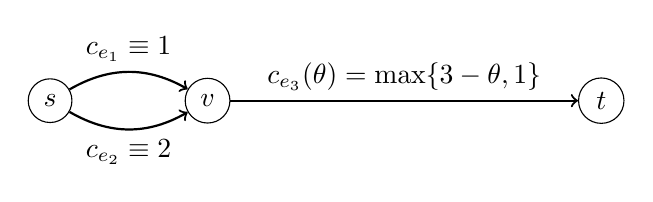
\begin{tikzpicture}
        \node[draw,circle](0)at(0,1) {$s$};
        \node[draw,circle](1)at(2, 1) {$v$};
        \node[draw,circle](2)at(7,1) {$t$};
        
        \draw[thick,->, bend left](0) to[bend left] node[above]{$c_{e_1}\equiv 1$} (1);
        \draw[thick,->](0) to[bend right] node[below]{$c_{e_2}\equiv 2$} (1);
        \draw[thick,->](1) --node[above]{$c_{e_3}(\theta) = \max\{ 3 - \theta, 1\}$} (2);
    \end{tikzpicture}
    \caption{Both $e_1$ and $e_2$ are active at time $0$ with $T_{e_2}(l_{s,s}(0))> l_{s,v}(0)$.}\label{fig:bottleneck}
\end{figure}

This leaves us with the question of how to find the rest of the active edges for general FIFO cost functions.
For the rest of this section, let $c:\R\rightarrow\R^E_{\geq0}$ be a continuous cost function following the FIFO rule with $\lim_{\theta\to-\infty} T_e(\theta) = -\infty$ for all $e\in E$.
Now we want to exploit that once we determined $l_{s,t}(\theta)$, we can do another run of the Dynamic Dijkstra Algorithm on the reverse graph $\rev{G} = (V, \rev{E})$ with $\rev{E}\coloneqq \{ \rev{e} = wv \mid e=vw\in E \}$ to compute the latest departure time starting from any node $v$ to arrive before or at time $l_{s,t}(\theta)$ at $t$.

We define the corresponding cost function $\tilde c$ as \[
    \tilde c : \R \rightarrow \R_{\geq0}^{\rev E}, \quad
    \tilde c_{\rev e}(\theta) \coloneqq - \minv{T_e}(-\theta) - \theta.
\]
Note, that $T_e  \geq \id_\R$ and by Proposition~\ref{prop:reversal-props}~\ref{prop:reversal-props:flip-id} we infer $\minv{T_e} \leq \id_\R$.
Therefore, we have $\minv{T_e}(-\theta) \leq -\theta$ and thus $\tilde c_{\rev e}(\theta) \geq 0$.

We denote the traversal times induced by $\tilde c$ by $\tilde T_{\rev e}$ and $\tilde T_{\rev P}$,where $\rev P = \rev{e_k} \, \cdots \, \rev{e_1}$ for $P = e_1\,\cdots\, e_k$,
and the earliest arrival time due to $\tilde c$ as $\tilde l_{v,w}$.
The traversal times fulfill $\tilde T_e = -\minv{T_e}(-\theta)$ which is by Proposition~\ref{prop:reversal-props}~\ref{prop:reversal-props:continuous} strictly increasing.
Hence, $\tilde c$ follows the strong FIFO rule.
For a path $\rev{P} = \rev{e_k}\,\cdots\, \rev{e_1}$ the traversal time yields
\[
    \tilde T_{\rev P} (\theta)
    = \tilde T_{\rev{e_{k-1}}\,\cdots\,\rev{e_1}}(- \minv{T_{e_k}} ( - \theta ))
    = \tilde T_{\rev{e_{k-2}}\,\cdots\,\rev{e_1}}(-\minv{T_{e_{k-1}}} (\minv{T_{e_k}} ( - \theta ))
    = \cdots
    = - \minv{T_P}(-\theta)
\]
and the earliest arrival times are of the form
\[
    \tilde l_{v,w}(\theta)
    = \min_{P\in\paths_{w,v}} \tilde T_{\rev{P}}(\theta)
    = \min_{P\in\paths_{w,v}} - \minv{T_P}(-\theta)
    = - \max_{P\in\paths_{w,v}} \minv{T_P}(-\theta)
    = - \minv{l_{w,v}}(-\theta)
\]

With this setup, we can do a second run of the Dynamic Dijkstra Algorithm to obtain the vector \[
    (\tilde l_{t,w}( - l_{s,t}(\theta) ))_w = (- \minv{l_{t,w}}( l_{s,t}(\theta) ))_w.
\]
Using Lemma~\ref{lem:characterization-active-edges} we can now check whether an outgoing edge $sw\in\outEdges{s}$ of $s$ is active at time $\theta$ by evaluating $T_e(\theta) \leq \minv{l_{t,w}}( l_{s,t}(\theta))$.

\begin{algorithm}[ht]
    \begin{minted}[mathescape, linenos]{python}
def get_active_edges(
  costs: List[PiecewiseLinear], theta: float, source: Node, sink: Node,
  relevant_nodes: Set[Node], graph: DirectedGraph, strong_fifo: bool
) -> Set[Edge]:
  if len(source.outgoing_edges) <= 1:
    return source.outgoing_edges
  arrivals = dynamic_dijkstra(
    theta, source, sink, relevant_nodes, costs
  )
  if strong_fifo:
    return backtrack_shortest_paths(costs, arrivals, source, sink)
  else: # Second run of Dijkstra on the reverse graph.
    graph.reverse()
    traversals = [cost + identity for cost in costs]
    new_costs: List[Callable[[float], float]] = [
      lambda t: -trav.reversal(-t) - t for trav in traversals
    ]
    neg_departures = dynamic_dijkstra(
      -arrivals[sink], sink, source, relevant_nodes, new_costs
    )
    graph.reverse()
    return [
      e for e in source.outgoing_edges
      if traversals[e.id](theta) <= -neg_departures[e.node_to]
    ]
  \end{minted}
  \caption{Calculating Active Edges}
  \label{alg:calculate-active-edges}
\end{algorithm}


To implement this algorithm, we have to restrict ourselves to cost functions where the reversal of $T_e$ can be evaluated easily.
This is the case, for example, if $c_e$ are piecewise linear functions.
The resulting algorithm for this class of functions can be seen in Algorithm~\ref{alg:calculate-active-edges}.
Here, the flag \code{strong_fifo} is expected to be set only for cost functions following the strong FIFO rule.
For these type of functions, we use the simpler backtracking search; for  general FIFO functions, we use the approach described above.
Other than that, if $s$ has only up to one outgoing edge, we simply return $\outEdges{s}$.
